\documentclass[a0,portrait]{a0poster}

\usepackage[T1]{fontenc}                    % Ausgabekodierung
\usepackage[utf8]{inputenc}                 % Eingabekodierung
\usepackage[english]{babel}                 % Deutsch 

\usepackage{amsmath,amssymb,amsthm} % Math
\usepackage{stmaryrd,multicol}               % Lightning

\pagestyle{empty}
\setcounter{secnumdepth}{0}

\usepackage{xcolor}
\definecolor{oceangreen}{RGB}{0,75,90}

\usepackage{tikz}
\tikzstyle{vertex} = [circle, draw, fill=oceangreen!10,
  inner sep=2pt, minimum width=40pt]

\usepackage[absolute]{textpos}
\usepackage{graphicx}
\usepackage{fancybox}
\usepackage{wrapfig,times}
\usepackage{url}

% see documentation for a0poster class for the size options here
\let\Textsize\normalsize
\def\Head#1{\noindent\hbox to \hsize{\hfil{\LARGE\color{oceangreen} #1}}\bigskip}
\def\LHead#1{\noindent{\LARGE\color{oceangreen} #1}\smallskip}
\def\Subhead#1{\noindent{\large\color{oceangreen} #1}}
\def\Title#1{\noindent{\VeryHuge\color{oceangreen!90} #1}}

\TPGrid[40mm,40mm]{15}{25}  % 3 - 1 - 7 - 1 - 3 Columns

\parindent=0pt
\parskip=0.5\baselineskip

\newcommand{\block}[1]{
\colorbox{oceangreen!10}{\parbox{\linewidth}{\vspace{0.5em}{\noindent #1}\vspace{0.25em}}}
}

% \textblockcolor{yellow}

\begin{document}

\begin{textblock}{12}(0,-0.25)
\resizebox{!}{1.5\TPVertModule}{\includegraphics{ispunienfor.pdf}}
\end{textblock}

\begin{textblock}{2}(14,0.25)
\resizebox{!}{\TPVertModule}{\includegraphics{logoispcmyk.pdf}}
\end{textblock}

\begin{textblock}{17}(-1,1.5)
\block{
\VeryHuge
\color{oceangreen}
\hspace{1\TPHorizModule}State-Based Routing for Computational Sustainability
}
\end{textblock}

\begin{textblock}{17}(-1,25.5)
\block{
\color{oceangreen}
\hspace{1\TPHorizModule}
Ren\'e Sch\"onfelder (\texttt{schoenfr@isp.uni-luebeck.de})
\hspace{3ex}and\hspace{3ex}Martin Leucker (\texttt{leucker@isp.uni-luebeck.de}),
\hfill July 6, 2012 \hspace{1\TPHorizModule}
}
\end{textblock}

\begin{textblock}{5}(0,2.5)
\LHead{Introduction} \\
Various routing models each considering some aspects of finding ``best''
solutions:
\begin{itemize}
  \item Shortest Path Problem: Finding a shortest path also yields an efficient path regarding energy consumption.
  \item Shortest Weight-Constrained Path Problem: Optimize more than one target function, e.g.\ time and energy-consumption.
  \item Time-Dependent and Multi-Modal Routing: Finding shortest paths depending on the time, caused for example by including public transportation.
  \item Energy-Optimal Routing: Considering energy constraints for electric vehicles.
  \item Stochastic Routing: Minimizing expected costs, maybe given certain conditional probabilities.
  \item Rerouting: After finding an efficient path and turning to a different direction (or gaining additional information),
  quickly find an alternate efficient route.
\end{itemize}
Each model comes with its own set of algorithms,
our aim is to find a model unifying some aspects while still
allowing for most algorithms known for the shortest path problem.
\end{textblock}

\begin{textblock}{5}(0,8.25)
\LHead{Prototype} \\
The Technische Universit\"at M\"unchen (TUM) developed a prototypic routing service,
which is further developed at the University of L\"ubeck,
available at \url{www.isp.uni-luebeck.de/greennav}. It is used
to evaluate different routing algorithms. You can see a range prediction
of an electric vehicle.\\[1em]
\resizebox{5\TPHorizModule}{!}{\includegraphics{greennav.png}}
\end{textblock}

\begin{textblock}{5}(0,14.75)
\LHead{Definition: State-Based Routing}
\begin{itemize}
  \item $G = (V, E)$ is a graph,
  \item $S$ is a set of states preordered by $\leq_S$,
  \item $\mathcal S:\ V \to \mathcal P(S)$ describes possible states at each vertex,
  \item $\mathbb W$ is a set of \emph{monotone} ($x_1 \leq_S x_2 \to f(x_1) \leq_S f(x_2)$)
  and \emph{extensive} ($x \leq_S f(x)$) weights $S \leadsto S$,
  \item $\mathcal W':\ E \to \mathbb W$ is a weighting,
\end{itemize}
such that
\begin{itemize}
  \item $\mathcal W'(x, y)$ is a weight $\mathcal S(x) \to \mathcal S(y)$, and
  \item the \emph{extension} of $\mathcal W'$ again is $\mathcal W:\ \text{walks} \to \mathbb W$ given by
  \[\mathcal W(\gamma) = \mathcal W'(v_0, v_1) \circ \ldots \circ \mathcal W'(v_{k-1}, v_k)\]
  for all walks $\gamma = (v_0, \ldots, v_k), k \geq 0$ (identity for $k = 0$).
\end{itemize}
\vspace{0.5em}
Objective:
\begin{itemize}
  \item Given $x, y \in V$ and initial state $s \in \mathcal S(x)$,
  find at least one corresponding path
  for each minimal element in $\min(\mathcal W(\text{walks from}\ x\ \text{to}\ y)(s))$
  (except for equivalence), where
  \[\min(S) := \{s \in S\ |\ \neg\exists s' \in S:\ s' < s\}.\]
\end{itemize}
\end{textblock}

\begin{textblock}{5}(5.5,17)
\LHead{Relation to Time-Dependent Routing} \\
Using a total order (or total preorder) the state-based routing problem is almost
equivalent to time-dependent routing. Time-dependency is realized mainly
by two changes to the common shortest path problem:
\begin{itemize}
  \item Edge costs $f: \mathbb R \to \mathbb R_{+}$ are functions from departure times to
  time costs.
  \item FIFO property: $x_1 + f(x_1) \leq x_2 + f(x_2)$ for all $x_1 \leq x_2$.
\end{itemize}
Given an edge cost function $f$, we can define an appropriate $g$ with
$g(x) = x + f(x)$, i.e.\ considering the \emph{arrival time}, such that
\begin{itemize}
  \item $g$ is extensive, because $f$ is non-negative, and
  \item $g$ is monotone due to the FIFO property.
\end{itemize}
Thus time-dependent routing is a special case of state-based routing.
\end{textblock}

\begin{textblock}{5}(5.5,2.5)
\LHead{Energy Constraints} \\
The set of states consists of battery charges in $B := [0, K] \cup \{-\infty\}$
(and altitudes):
\begin{itemize}
  \item Maximum capacity $K > 0$
  \item Initial charge $J \in [0, K]$
  \item Recuperation (regaining energy)
  \item Can not drive with an empty battery
\end{itemize}
Example:
\begin{center}
\vspace{-1em}
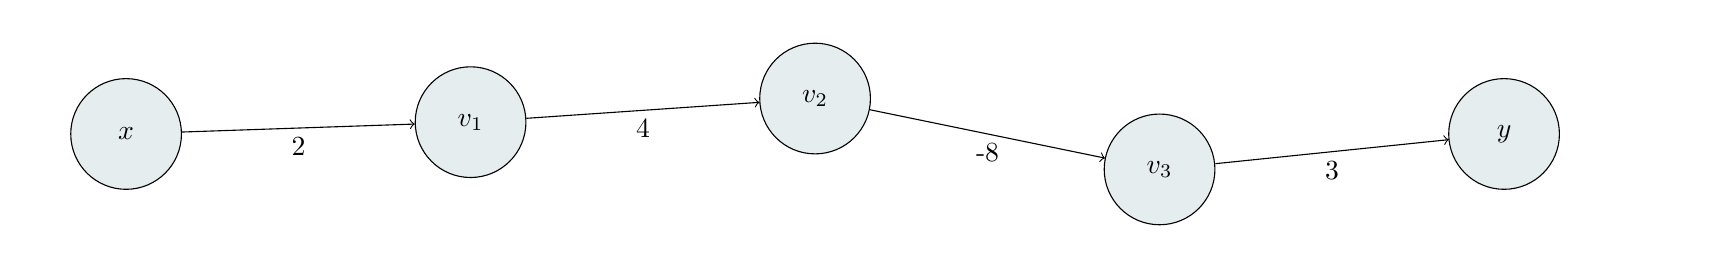
\begin{tikzpicture}[xscale=2.5, yscale=1.5,auto,swap]
  \clip (0.5,0) rectangle (9, 1.9);
  %\draw[color=oceangreen!20!white] (0,0) rectangle (9, 2);

  \node[vertex] (x) at (1, 1) {$x$};
  \node[vertex] (a) at (2.75, 1.1) {$v_1$};
  \node[vertex] (b) at (4.5, 1.3) {$v_2$};
  \node[vertex] (c) at (6.25, 0.7) {$v_3$};
  \node[vertex] (y) at (8, 1) {$y$};

  \path[draw,->] (x) -- node[below] {2} (a);
  \path[draw,->] (a) -- node[below] {4} (b);
  \path[draw,->] (b) -- node[below] {-8} (c);
  \path[draw,->] (c) -- node[below] {3} (y);
%  \path[draw,thick,blue,->]<4-> (e) -- node {2} (f);
\end{tikzpicture}
\end{center}
\vspace{-0.5em}
Battery transformation function of given path:
\begin{center}
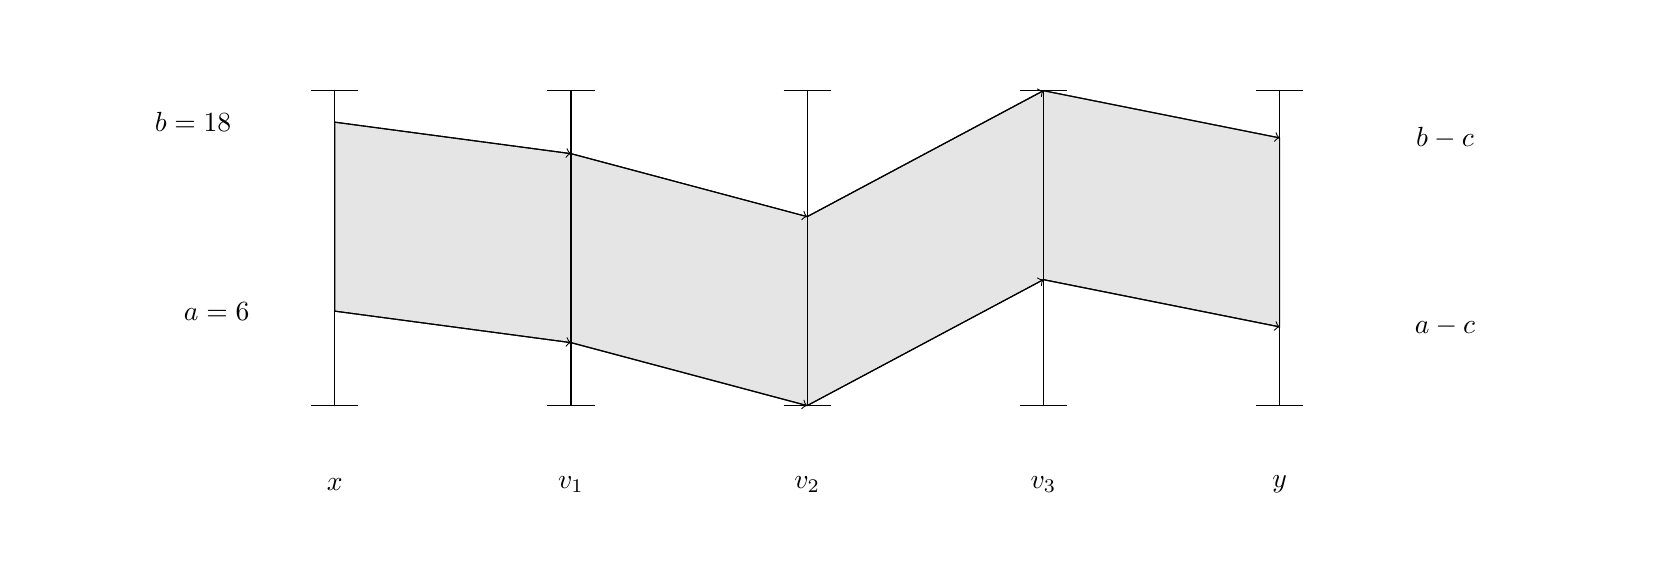
\begin{tikzpicture}[xscale=3,yscale=2,auto,swap]
  \clip (-0.3,-0.9) rectangle (6.5, 2.4);
  %\draw[color=oceangreen!20!white] (0,-0.9) rectangle (6, 2.4);
  \filldraw[fill=black!10]
    (1,1.8) -- (2,1.6) -- (3,1.2) -- (4, 2) -- (5, 1.7) --
    (5,0.5) -- (4,0.8) -- (3,0) -- (2, 0.4) -- (1, 0.6) -- cycle;
  
  \path[draw] (1, 0) -- (1, 2);
  \path[draw] (0.9, 0) -- (1.1, 0);
  \path[draw] (0.9, 2) -- (1.1, 2);
  \path[draw] (2, 0) -- (2, 2);
  \path[draw] (1.9, 0) -- (2.1, 0);
  \path[draw] (1.9, 2) -- (2.1, 2);
  \path[draw] (3, 0) -- (3, 2);
  \path[draw] (2.9, 0) -- (3.1, 0);
  \path[draw] (2.9, 2) -- (3.1, 2);
  \path[draw] (4, 0) -- (4, 2);
  \path[draw] (3.9, 0) -- (4.1, 0);
  \path[draw] (3.9, 2) -- (4.1, 2);
  \path[draw] (5, 0) -- (5, 2);
  \path[draw] (4.9, 0) -- (5.1, 0);
  \path[draw] (4.9, 2) -- (5.1, 2);

  \node (x) at (1, -0.5) {$x$};
  \node (c) at (2, -0.5) {$v_1$};
  \node (e) at (3, -0.5) {$v_2$};
  \node (f) at (4, -0.5) {$v_3$};
  \node (y) at (5, -0.5) {$y$};

  \node at (0.4, 1.8) {$b = 18$};
  \path[draw, ->] (1, 1.8) -- (2, 1.6);
  \path[draw, ->] (2, 1.6) -- (3, 1.2);
  \path[draw, ->] (3, 1.2) -- (4, 2);
  \path[draw, ->] (4, 2) -- (5, 1.7);
  \node at (5.7, 1.7) {$b - c$};
  \node at (0.5, 0.6) {$a = 6$};
  \path[draw, ->] (1, 0.6) -- (2, 0.4);
  \path[draw, ->] (2, 0.4) -- (3, 0);
  \path[draw, ->] (3, 0) -- (4, 0.8);
  \path[draw, ->] (4, 0.8) -- (5, 0.5);
  \node at (5.7, 0.5) {$a - c$};
\end{tikzpicture}
\end{center}
Battery charge more than $b = 18$ energy units are wasted.
Having less than $a = 6$ energy units renders this path useless.
The overall costs are $c = 2 + 4 - 8 + 3 = 1$.
\end{textblock}

\begin{textblock}{5}(5.5,9)
\LHead{State-Based Profile Search} \\
As it was done for the time-dependent routing problem,
we may consider the problem of finding optimal solutions
for each possible starting state. In terms of energy constraints,
one path may be more efficient than another path, if able to invest
a higher amount of battery charge.
\begin{center}
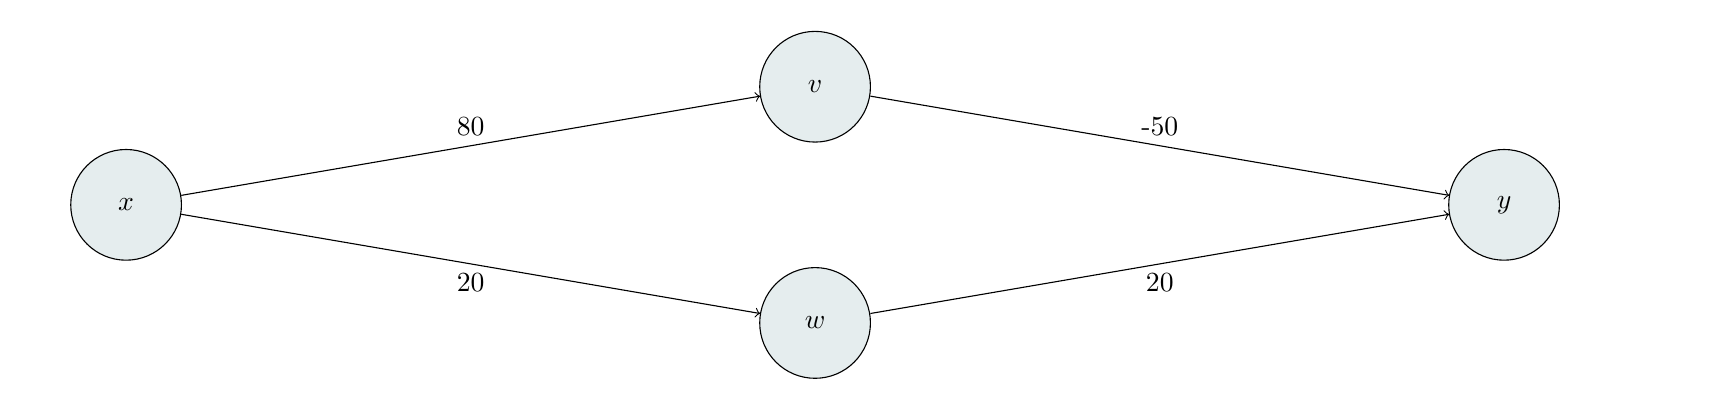
\begin{tikzpicture}[xscale=2.5, yscale=1.5,auto,swap]
  \clip (0.5,-0.5) rectangle (9, 2.5);
  \node[vertex] (x) at (1, 1) {$x$};
  \node[vertex] (w) at (4.5, 0) {$w$};
  \node[vertex] (v) at (4.5, 2) {$v$};
  \node[vertex] (y) at (8, 1) {$y$};

  \path[draw,->] (x) -- node[below] {20} (w);
  \path[draw,->] (w) -- node[below] {20} (y);
  \path[draw,->] (x) -- node[above] {80} (v);
  \path[draw,->] (v) -- node[above] {-50} (y);
\end{tikzpicture}
\end{center}
\begin{itemize}
  \item $xvy$ less costs (30), but requires $J \geq 80$,
  \item $xwy$ higher costs (40), but is possible with $J \geq 40$.
\end{itemize}
An optimal solution, called a \emph{policy}, therefore maps battery charges
$J \geq 80$ to $xvy$, all $40 \leq J < 80$ to $xwy$ and all other $J$ to no path.

Therefore, combining both functions by maximizing the energy value may
yield a non-trivial cost function:
\begin{center}
\begin{tikzpicture}[scale=1.5, auto, swap]
\tikzstyle{vertex} = [circle, draw, fill=oceangreen!10,
  inner sep=2pt, minimum width=10pt]
  \clip (-1,0) rectangle (11,9.1);
  \node at (1, 0.6) {$0$};
  \draw (2.5, 1) -- (9.5, 1);
  \draw (1, 1.5) -- (1, 8.5);
  \draw[dotted] (1, 1) -- (2.5, 1);
  \draw[dotted] (1, 1) -- (1, 1.5);
  \draw[dotted] (9.5, 1) -- (10, 1);
  \draw[dotted] (1, 8.5) -- (1, 9);
  \draw[dashed] (1, 1) -- (9, 9);
  % p'
  \node at (2.5, 0.65) {$h$};
  \draw (2.5, 1.1) -- (2.5, 0.9);
  % p' + K
  \node at (9.5, 0.65) {$h + K$};
  \draw (9.5, 1.1) -- (9.5, 0.9);
  % p''
  \node at (0, 1.5) {$h'$};
  \draw (0.9, 1.5) -- (1.1, 1.5);
  % p'' + K
  \node at (-0.1, 8.5) {$h' + K$};
  \draw (0.9, 8.5) -- (1.1, 8.5);
  \node[vertex, fill=black] (closed1) at (5, 4.5) {};
  \draw (closed1) -- (6, 5.5) -- (7, 5.5);
  \draw[dotted] (7, 5.5) -- (9.5, 5.5);
  \node[vertex, fill=black] (closedk2) at (9.5, 6.5) {};
  \node[vertex, fill=black] (closed2) at (4, 2.5) {};
  \node[vertex, fill=white] (open2) at (5, 3.5) {};
  \draw (closed2) -- (open2.south west);
  \draw[dotted] (open2.north east) -- (7, 5.5);
  \draw (7, 5.5) -- (8, 6.5) -- (closedk2);
\end{tikzpicture}
\end{center}
\end{textblock}

\begin{textblock}{4}(11,2.5)
\LHead{Stochasticity} \\
A direct generalization of energy-constraints using stochasticity is done
by modeling the battery charge as a random variable
\[J:\ \Omega \to B \qquad (\text{with}\ B = [0, K] \cup \{-\infty\}).\]
The edge cost functions then are random variables itself
$\Omega \to (B \to B)$, which can be formalized as a state transformation
function as $(\Omega \to B) \to (\Omega \to B)$ using the same $\omega \in \Omega$.

The questionable decision is the choice of the partial preorder $\leq$.
Two approaches are $J_1 \leq J_2$, if and only if
\begin{align}
\mathbb E(J_1\ |\ J_1 > -\infty) &\geq \mathbb E(J_2\ |\ J_2 > -\infty), \\
P(J_1 \geq c) &\geq P(J_2 \geq c), \quad c \in [0, K].
\end{align}
The former approach (1) yields non-monotone functions and thus does not fit
our state-based approach. The latter (2) is an adaptation from Uludag et al. \cite{Uludag2009}
and actually fits the state-based approach quite smoothly.
\end{textblock}

\begin{textblock}{4}(11,8)
\LHead{Algorithm Design} \\
The computational problem here arises from the fact, that an optimal solution
depends on the initial state. This renders a backward search impossible without
doing a profile search. The same goes for almost all precomputation methods.

However, by considering the profile search, we may use existing algorithms
with minor modifications as was shown for example by
Eisner et al.\ \cite{Eisner2011}.
The general concept for modifying existing algorithms is to use a partial
order queue and to reconsider the stop condition.

\begin{figure}[htp]
\centering
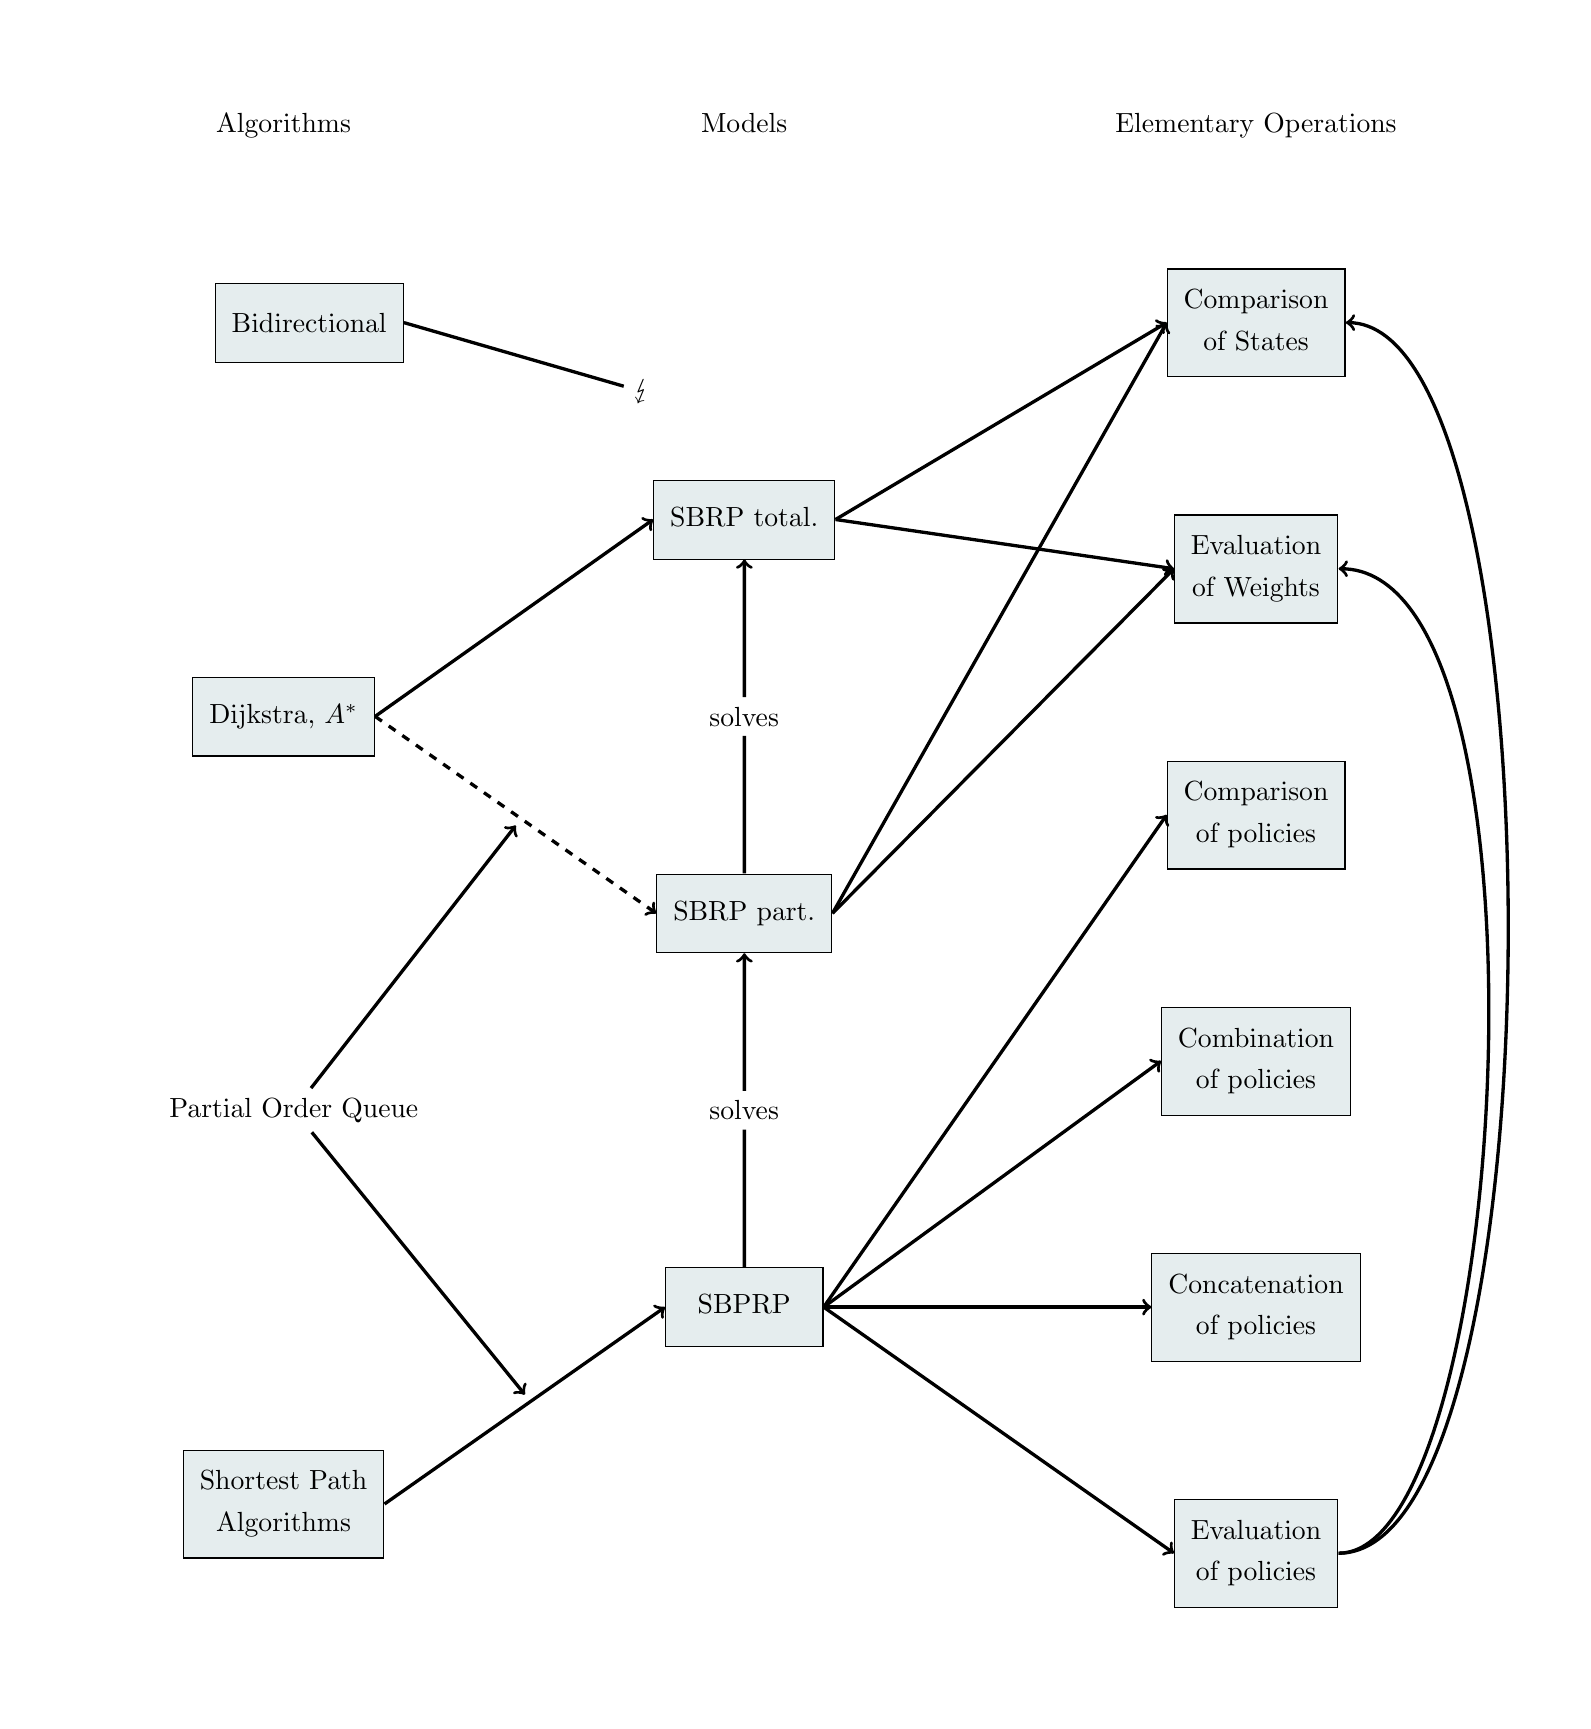
\begin{tikzpicture}[xscale=1.3, yscale=1.25, auto]
  \tikzstyle{box} = [rectangle, draw, fill=oceangreen!10,
  inner sep=6pt, minimum width=2cm, minimum height=1cm]
  \clip (0,0) rectangle (15,17);
  \node at (2.5, 16) {Algorithms\strut};
  \node at (7, 16) {Models\strut};
  \node at (12, 16) {Elementary Operations\strut};
  \node[box] (dij) at (2.5, 10) {Dijkstra, $A^{*}$};
  \node[box] (bidi) at (2.75, 14) {Bidirectional};
  \node (poq) at (2.6, 6) {Partial Order Queue};
  \node[box] (a) at (2.5, 2) {\shortstack{Shortest Path\strut \\ Algorithms\strut}};
  \node[box] (sbspptot) at (7, 12) {SBRP total.\strut};
  \node[box] (sbspppar) at (7, 8) {SBRP part.\strut};
  \node[box] (sbprp) at (7, 4) {SBPRP\strut};
  \node (solv1) at (7, 10) {solves};
  \draw[->, very thick] (solv1) -- (sbspptot);
  \draw[very thick] (solv1) -- (sbspppar);
  \node (solv2) at (7, 6) {solves};
  \draw[->, very thick] (solv2) -- (sbspppar);
  \draw[very thick] (solv2) -- (sbprp);
  \draw[->, very thick] (dij.east) -- (sbspptot.west);
  \draw[dashed, ->, very thick] (dij.east) -- (sbspppar.west) node[pos=0.5, below=0pt] (abc1) {};
  \draw[->, very thick] (a.east) -- (sbprp.west) node[pos=0.5, above=0pt] (abc2) {};
  \node (l1) at (6, 13.3) {$\lightning$};
  \draw[very thick] (bidi.east) -- (l1);
  \draw[->, very thick] (poq) -- (abc1.center);
  \draw[->, very thick] (poq) -- (abc2.center);
  \node[box] (compstates) at (12, 14) {\shortstack{Comparison\strut \\ of States\strut}};
  \node[box] (evalweights) at (12, 11.5) {\shortstack{Evaluation\strut \\ of Weights\strut}};
  \node[box] (comppolicy) at (12, 9) {\shortstack{Comparison\strut \\ of policies\strut}};
  \node[box] (combpolicy) at (12, 6.5) {\shortstack{Combination\strut \\ of policies\strut}};
  \node[box] (concpolicy) at (12, 4) {\shortstack{Concatenation\strut \\ of policies\strut}};
  \node[box] (evalpolicy) at (12, 1.5) {\shortstack{Evaluation\strut \\ of policies\strut}};
  \draw[->, very thick] (evalpolicy.east) .. controls (15,1.5) and (15,14) .. (compstates.east);
  \draw[->, very thick] (evalpolicy.east) .. controls (14.5,1.5) and (15,11.5) .. (evalweights.east);
  \draw[->, very thick] (sbspptot.east) -- (compstates.west);
  \draw[->, very thick] (sbspptot.east) -- (evalweights.west);
  \draw[->, very thick] (sbspppar.east) -- (compstates.west);
  \draw[->, very thick] (sbspppar.east) -- (evalweights.west);
  \draw[->, very thick] (sbprp.east) -- (comppolicy.west);
  \draw[->, very thick] (sbprp.east) -- (combpolicy.west);
  \draw[->, very thick] (sbprp.east) -- (concpolicy.west);
  \draw[->, very thick] (sbprp.east) -- (evalpolicy.west);
\end{tikzpicture}
\end{figure}
In contrast to priority queues, partial order queues provide two
essential functions:
\begin{itemize}
  \item \textbf{min} - to find any minimal object, and
  \item \textbf{front} - to query the set of all minimal objects.
\end{itemize}
\end{textblock}

\begin{textblock}{4}(11,17.2)
\LHead{Conclusions and Future Work} \\
First tests yielded reasonable results, but we just started to implement
various shortest path algorithms for the state-based routing problem and
its profile version. Hence runtime and space analyzations are near future
goals. The model itself is promising, comprising time-dependent routing,
battery constraints, stochasticity and multi-criteria routing, but the
running time is an important question to answer soon.

In the long run we aim to extend GreenNav by more sophisticated algorithms
and services. An egoistic routing algorithm is but the first step towards
ecological sustainability. Multi-modality and stochasticity are two important
points to consider.
\end{textblock}

\begin{textblock}{15}(0,20.9)
\line(1,0){2160}
\end{textblock}

\begin{textblock}{15}(0,21)
\begin{multicols}{3}
\renewcommand{\refname}{\normalfont\LHead{Related Work}\vspace{-1cm}}
\nocite{*}
\bibliographystyle{plain} %plain
\bibliography{ref}
\end{multicols}
\end{textblock}

\end{document}